\section{1. Leitungscodes}
\paragraph{Aufgabe 1.1:}
	Kodieren Sie den angegebene Bitsequenz mittels normalem Manchester-Code und geben Sie die resultierenden Signalfolge an.

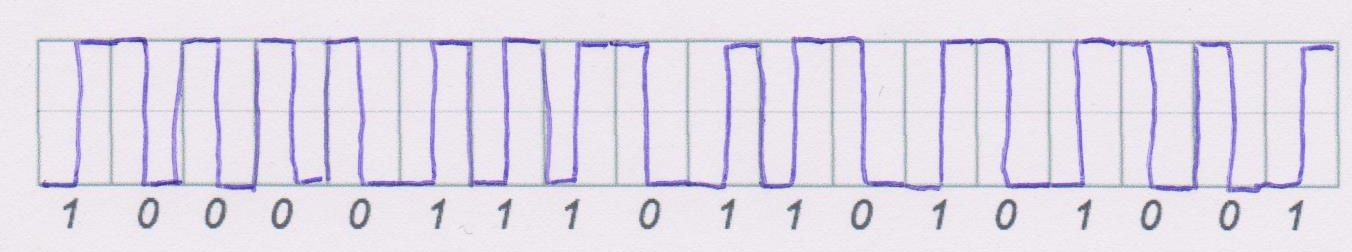
\includegraphics[scale=0.2]{blatt3_1_1}
\paragraph{Aufgabe 1.2:}
	Kodieren Sie den angegebene Bitsequenz mittels differentiellem Manchester-Code und geben Sie die resultierenden Signalfolge an. Gibt es eine eindeutige Lösung ?
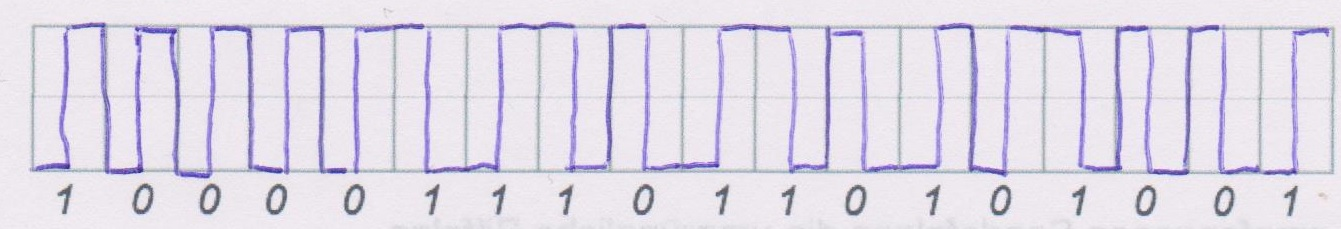
\includegraphics[scale=0.2]{blatt3_1_2}

\paragraph{Aufgabe 1.3:}
	Diskutieren und vergleichen (Tip: Rauschen) Sie kurz die Eigenschaften der beiden Leitungscodes.
\paragraph{Antwort:}
\section{2. Codemultiplex}
\paragraph{Aufgabe 1.1:}
	Berechnen Sie die zu sendenden Sendefolgen.
\paragraph{Antwort:} Die zu sendende Bitfolge ergibt sich aus der Addition beider Bitfolgen
	\begin{enumerate}

	\item Die Bitfolge für Empfänger $3$
		\\ 1: $-1\mid -1\mid +1\mid +1\mid -1\mid -1\mid +1\mid +1$
		\\ 0: $+1\mid +1\mid -1\mid -1\mid +1\mid +1\mid -1\mid -1$
		\\ 1: $-1\mid -1\mid +1\mid +1\mid -1\mid -1\mid +1\mid +1$
	\item Die Bitfolge für Empfänger $7$	
		\\ 1: $-1\mid -1\mid +1\mid +1\mid +1\mid +1\mid -1\mid -1$
		\\ 1: $-1\mid -1\mid +1\mid +1\mid +1\mid +1\mid -1\mid -1$
		\\ 0: $+1\mid +1\mid -1\mid -1\mid -1\mid -1\mid +1\mid +1$
	\item Die Addierte Bitfolge ist demnach
		\\$-1-1\mid -1-1\mid +1+1\mid +1+1\mid -1+1\mid -1+1\mid +1-1\mid +1-1 = -2\mid -2\mid +2\mid +2\mid 0\mid 0\mid 0\mid 0$
		\\$+1-1\mid +1-1\mid -1+1\mid -1+1\mid +1+1\mid +1+1\mid -1-1\mid -1-1 = 0\mid 0\mid 0\mid 0\mid +2\mid +2\mid -2\mid -2$
		\\$-1-1\mid -1-1\mid +1+1\mid +1+1\mid -1+1\mid -1+1\mid +1-1\mid +1-1 = -2\mid -2\mid +2\mid +2\mid 0\mid 0\mid 0\mid 0$
	\end{enumerate}
\paragraph{Aufgabe 1.2:}
	Berechnen Sie aus den empfangenen Sendefolgen die ursprüngliche Bitfolge.
\paragraph{Antwort:} Um die gesendeten Sendefolgen zu entschlüsseln müssen wir jetzt einfach das Skalarprodukt bilden.
	\begin{enumerate}
		\item Empfänger $4$
			\\$(-2\cdot 1)+(-2\cdot 1)+(2\cdot -1)+(2\cdot -1)+(0\cdot 1)+(0\cdot 1)+(0\cdot -1)+(0\cdot -1) = -8 \Rightarrow \text{gesendetes Bit: } 1$
			\\$(0\cdot 1)+(0\cdot 1)+(0\cdot -1)+(0\cdot -1)+(2\cdot 1)+(2\cdot 1)+(-2\cdot -1)+(-2\cdot -1) = 8 \Rightarrow \text{gesendetes Bit: } 0$
			\\$(-2\cdot 1)+(-2\cdot 1)+(2\cdot -1)+(2\cdot -1)+(0\cdot 1)+(0\cdot 1)+(0\cdot -1)+(0\cdot -1) = -8 \Rightarrow \text{gesendetes Bit: } 1$
		\item Empfänger $7$	
			\\$(-2\cdot 1)+(-2\cdot 1)+(2\cdot -1)+(2\cdot -1)+(0\cdot -1)+(0\cdot -1)+(0\cdot 1)+(0\cdot 1) = -8 \Rightarrow \text{gesendetes Bit: } 1$
			\\$(0\cdot 1)+(0\cdot 1)+(0\cdot -1)+(0\cdot -1)+(2\cdot -1)+(2\cdot -1)+(-2\cdot 1)+(-2\cdot 1) = -8 \Rightarrow \text{gesendetes Bit: } 1$
			\\$(-2\cdot 1)+(-2\cdot 1)+(2\cdot -1)+(2\cdot -1)+(0\cdot 1)+(0\cdot 1)+(0\cdot -1)+(0\cdot -1) = 8 \Rightarrow \text{gesendetes Bit: } 0$
	\end{enumerate}